\documentclass[12pt,a4paper]{scrartcl}
\usepackage[english]{babel}
\usepackage{natbib}
\bibliographystyle{agsm} % Harvard
%\bibliographystyle{alpha}
\usepackage{amsmath}
\usepackage{amsfonts}
\usepackage{amssymb}
\usepackage{fontspec}
\setmainfont[
    Ligatures=TeX,
    Numbers={OldStyle, Proportional}
]{DejaVu Sans}
\setsansfont[
    Ligatures=TeX,
    Numbers={OldStyle, Proportional}
]{DejaVu Sans}
\setmonofont[
    Ligatures=TeX,
    Numbers={OldStyle, Proportional}
]{DejaVu Sans Mono}
\usepackage{makeidx}
\makeindex
\usepackage{graphicx}
\usepackage{xcolor}
%\usepackage{termcol}
%\loadcolors{terminalcolors}
\definecolor{BackgroundColour}{RGB}{241,239,238}
\definecolor{ForegroundColour}{RGB}{104,97,94}
\definecolor{CursorColour}{RGB}{104,97,94}
\definecolor{Black}{RGB}{27,25,24}
\definecolor{BoldBlack}{RGB}{118,110,107}
\definecolor{Red}{RGB}{242,44,64}
\definecolor{BoldRed}{RGB}{242,44,64}
\definecolor{Green}{RGB}{90,183,56}
\definecolor{BoldGreen}{RGB}{90,183,56}
\definecolor{Yellow}{RGB}{213,145,26}
\definecolor{BoldYellow}{RGB}{213,145,26}
\definecolor{Blue}{RGB}{64,126,231}
\definecolor{BoldBlue}{RGB}{64,126,231}
\definecolor{Magenta}{RGB}{102,102,234}
\definecolor{BoldMagenta}{RGB}{102,102,234}
\definecolor{Cyan}{RGB}{0,173,156}
\definecolor{BoldCyan}{RGB}{0,173,156}
\definecolor{White}{RGB}{168,161,159}
\definecolor{BoldWhite}{RGB}{241,239,238}

%base16/atelierforest.light
%xcolors.net/euphrasia
%collection/hund
%collection/dawn

\usepackage{listings}
\lstset{
	frame=none,
%	aboveskip=3mm,
%	belowskip=3mm,
	captionpos=b,
	showstringspaces=false,
	breaklines=true,
	breakatwhitespace=true,
	postbreak=\mbox{\textcolor{Red}{$\hookrightarrow$}\space},
%	tabsize=4,
	keepspaces=true,
	columns=fullflexible,
	escapeinside={\%*}{*)},
	otherkeywords={self},
	deletekeywords={},
	numbers=left,
	numbersep=5pt,
	numberstyle=\color{BackgroundColour!95!ForegroundColour},
	%% Colors and fonts:
	basicstyle=\footnotesize\ttfamily\color{ForegroundColour!70!BackgroundColour},
	numberstyle=\tiny\color{ForegroundColour},
	keywordstyle=\color{Blue},
	commentstyle=\color{BoldGreen},
    identifierstyle=\color{ForegroundColour},
	stringstyle=\color{Red},
	backgroundcolor=\color{BackgroundColour!95!ForegroundColour},
	rulecolor=\color{Black}
}
\usepackage[space=true]{accsupp}
\newcommand\emptyaccsupp[1]{\BeginAccSupp{ActualText={}}#1\EndAccSupp{}}
\usepackage{varioref}
\PassOptionsToPackage{hyphens}{url}\usepackage[colorlinks=true, linkcolor=Blue, citecolor=BoldYellow, plainpages=false, unicode, pdfencoding=auto ,backref=page]{hyperref}
\usepackage{cleveref}

%\setlength{\parindent}{0pt}
\pagecolor{BackgroundColour}
\color{ForegroundColour}

\author{Raphael Emberger}
\title{Kaggle-Challenge: San Francisco Crime Classification}
\date{\today}


\renewcommand{\theequation}{\Roman{equation}}
\makeindex
\newcommand{\inlinelisting}[1]{\colorbox{BackgroundColour!95!ForegroundColour}{\color{ForegroundColour!70!BackgroundColour}\lstinline[columns=fixed,language=python]{#1}}}
%\end{lstlisting} <- texmaker syntax highlight fix
\begin{document}
\begin{titlepage}
\centering
\begin{figure}[htbp]\label{f:san_francisco}
\includegraphics[width=\textwidth]{San-Francisco}\par\vspace{1cm}
\caption{\cite{sf_pic}}
\end{figure}
{\huge\bfseries Kaggle-Challenge: San Francisco Crime Classification\par}
\vspace{1.5cm}
{\scshape\LARGE Nagaoka University of Technology \par}
\vspace{2cm}
\begin{center}
\begin{tabular}{r l}
Date: & \today\\
Instructor: & Professor Yukawa
\end{tabular}
\end{center}
\vfill
{\Large\itshape Raphael Emberger\par}
\vfill
\end{titlepage}

\tableofcontents
\pagebreak

\section{Preface}\label{s:preface}
Firstly, I want to express my gratitude to Professor Yukawa for guiding me in this project and to the Kokusaika staff members to arrange my stay here at the Nagaoka University of Technology(subsequently referred to as "NUT").
I was given the generous opportunity to study at the NUT for one semester, for which I am very grateful. During that time I could choose from the following six Kaggle challenges to work on as project work:
\begin{itemize}
\item Toxic Comment Classification Challenge \citep{kgl_toxic_comment}
\item TalkingData AdTracking Fraud Detection Challenge \citep{kgl_talking_data}
\item Quora Question Pairs \citep{kgl_quora}
\item Expedia Hotel Recommendations \citep{kgl_expedia}
\item San Francisco Crime Classification \citep{kgl_sf_crime}
\item Inclusive Images Challenge \citep{kgl_inclusive_images}
\end{itemize}
Of those, I was most interested in the classification of reported crimes \citep{kgl_sf_crime}, as in my opinion this was an interesting challenge, given the dataset to be only consisting of time and spatial data. As such, this report is dedicated to take on this challenge.

\pagebreak
\section{Abstract}\label{s:abstract}
The first attempt to classify crimes based on date-time, district and coordinates was to build a neural network using \cite{keras}. This approach failed by remaining on the same level as always guessing the most prominent label("Larceny/Theft") - ~20\%. This reached rank 1058 out of 2335.

The second attempt reached better results. This time, finished projects for the same challenge were used as reference to find problems with the first approach. This time, a Bernoulli Naïve Bayes classifier was used on the binarized dataset and reached a log-loss of 2.464 or 26.02\%, which raised the rank up to 675.

The third and last attempt consisted of integrating the first attempt of using Keras into the second attempt. After some adjustment, the rank could be slightly improved once more: With a log-loss of 2.456(26.39\%), rank 664 could be claimed.

The time for more improvement was not available because too much time was wasted on the first attempt, but the next steps would have included data enrichment and data manipulation.

\pagebreak
\section{Introduction}\label{s:intro}
\subsection{Initial situation}\label{ss:initial_situation}
The challenge has been out since roughly 3 years and since then, many teams have participated and submitted their results. This lead the leader-board to fill up with 2335 submissions which were ranked and their results displayed online(see "Leaderboard" at \cite{kgl_sf_crime}). The results vary from 34.53877 up to 1.95936, where the sample submission with a value of 32.89183 reaches rank 2241(see \ref{ss:loss_function} for the ranking principle).

When searching on the internet for documents about that challenge, there are multiple such projects to be found. For example:
\begin{itemize}
\item A paper from \cite{slideshare_sf_crime_prediction}. 2 Naïve Bayes, Decision Tree, Random Forest and Support Vector Machines classifiers were used. Reached highest accuracy of 23.16\% with a Decision Tree.
\item A blog post from \cite{efavdb_sf_crime_prediction}. In that project, a Bernoulli Naïves Bayes classifier was used. Reached a log-loss score of 2.58.
\item A blog post from \cite{mattmurray_blog}. AdaBoost, Bagging, Extra Trees, Gradient Boosting, K-Nearest Neighbors, Random Forest classifiers and Logistic Regresson were used in this project. The dataset was enriched greatly by adding 9 other datasets (features like house prices, income, police and public transportation stations, healthcare center and homeless shelter locations, altitudes). Highest accuracy achieved with Gradient Boosted Trees, resulting in 45.7\%.
\end{itemize}

\subsection{Objective}\label{ss:objective}
The objective of this project is to produce a system that is capable of classifiying the type of crime based off of the provided data consisting of date time stamps, the name of the district and street as well as the coordinates of the registered report. To quote \cite{kgl_sf_crime}:

\begin{quote}
From 1934 to 1963, San Francisco was infamous for housing some of the world's most notorious criminals on the inescapable island of Alcatraz.

Today, the city is known more for its tech scene than its criminal past. But, with rising wealth inequality, housing shortages, and a proliferation of expensive digital toys riding BART to work, there is no scarcity of crime in the city by the bay.

From Sunset to SOMA, and Marina to Excelsior, this competition's dataset provides nearly 12 years of crime reports from across all of San Francisco's neighborhoods. Given time and location, you must predict the category of crime that occurred.

We're also encouraging you to explore the dataset visually. What can we learn about the city through visualizations like this Top Crimes Map? The top most up-voted scripts from this competition will receive official Kaggle swag as prizes. 
\end{quote}

Although the Kaggle challenge includes submitting an softmax array of the predictions of the test data, this objectives shifts towards self evaluation on the training set. The reason for this is that the challenge is already over and self evaluation was considered an easier approach to measure the success of the system.

\begin{center}
\begin{figure}[htbp]\label{f:sf_crime_map}
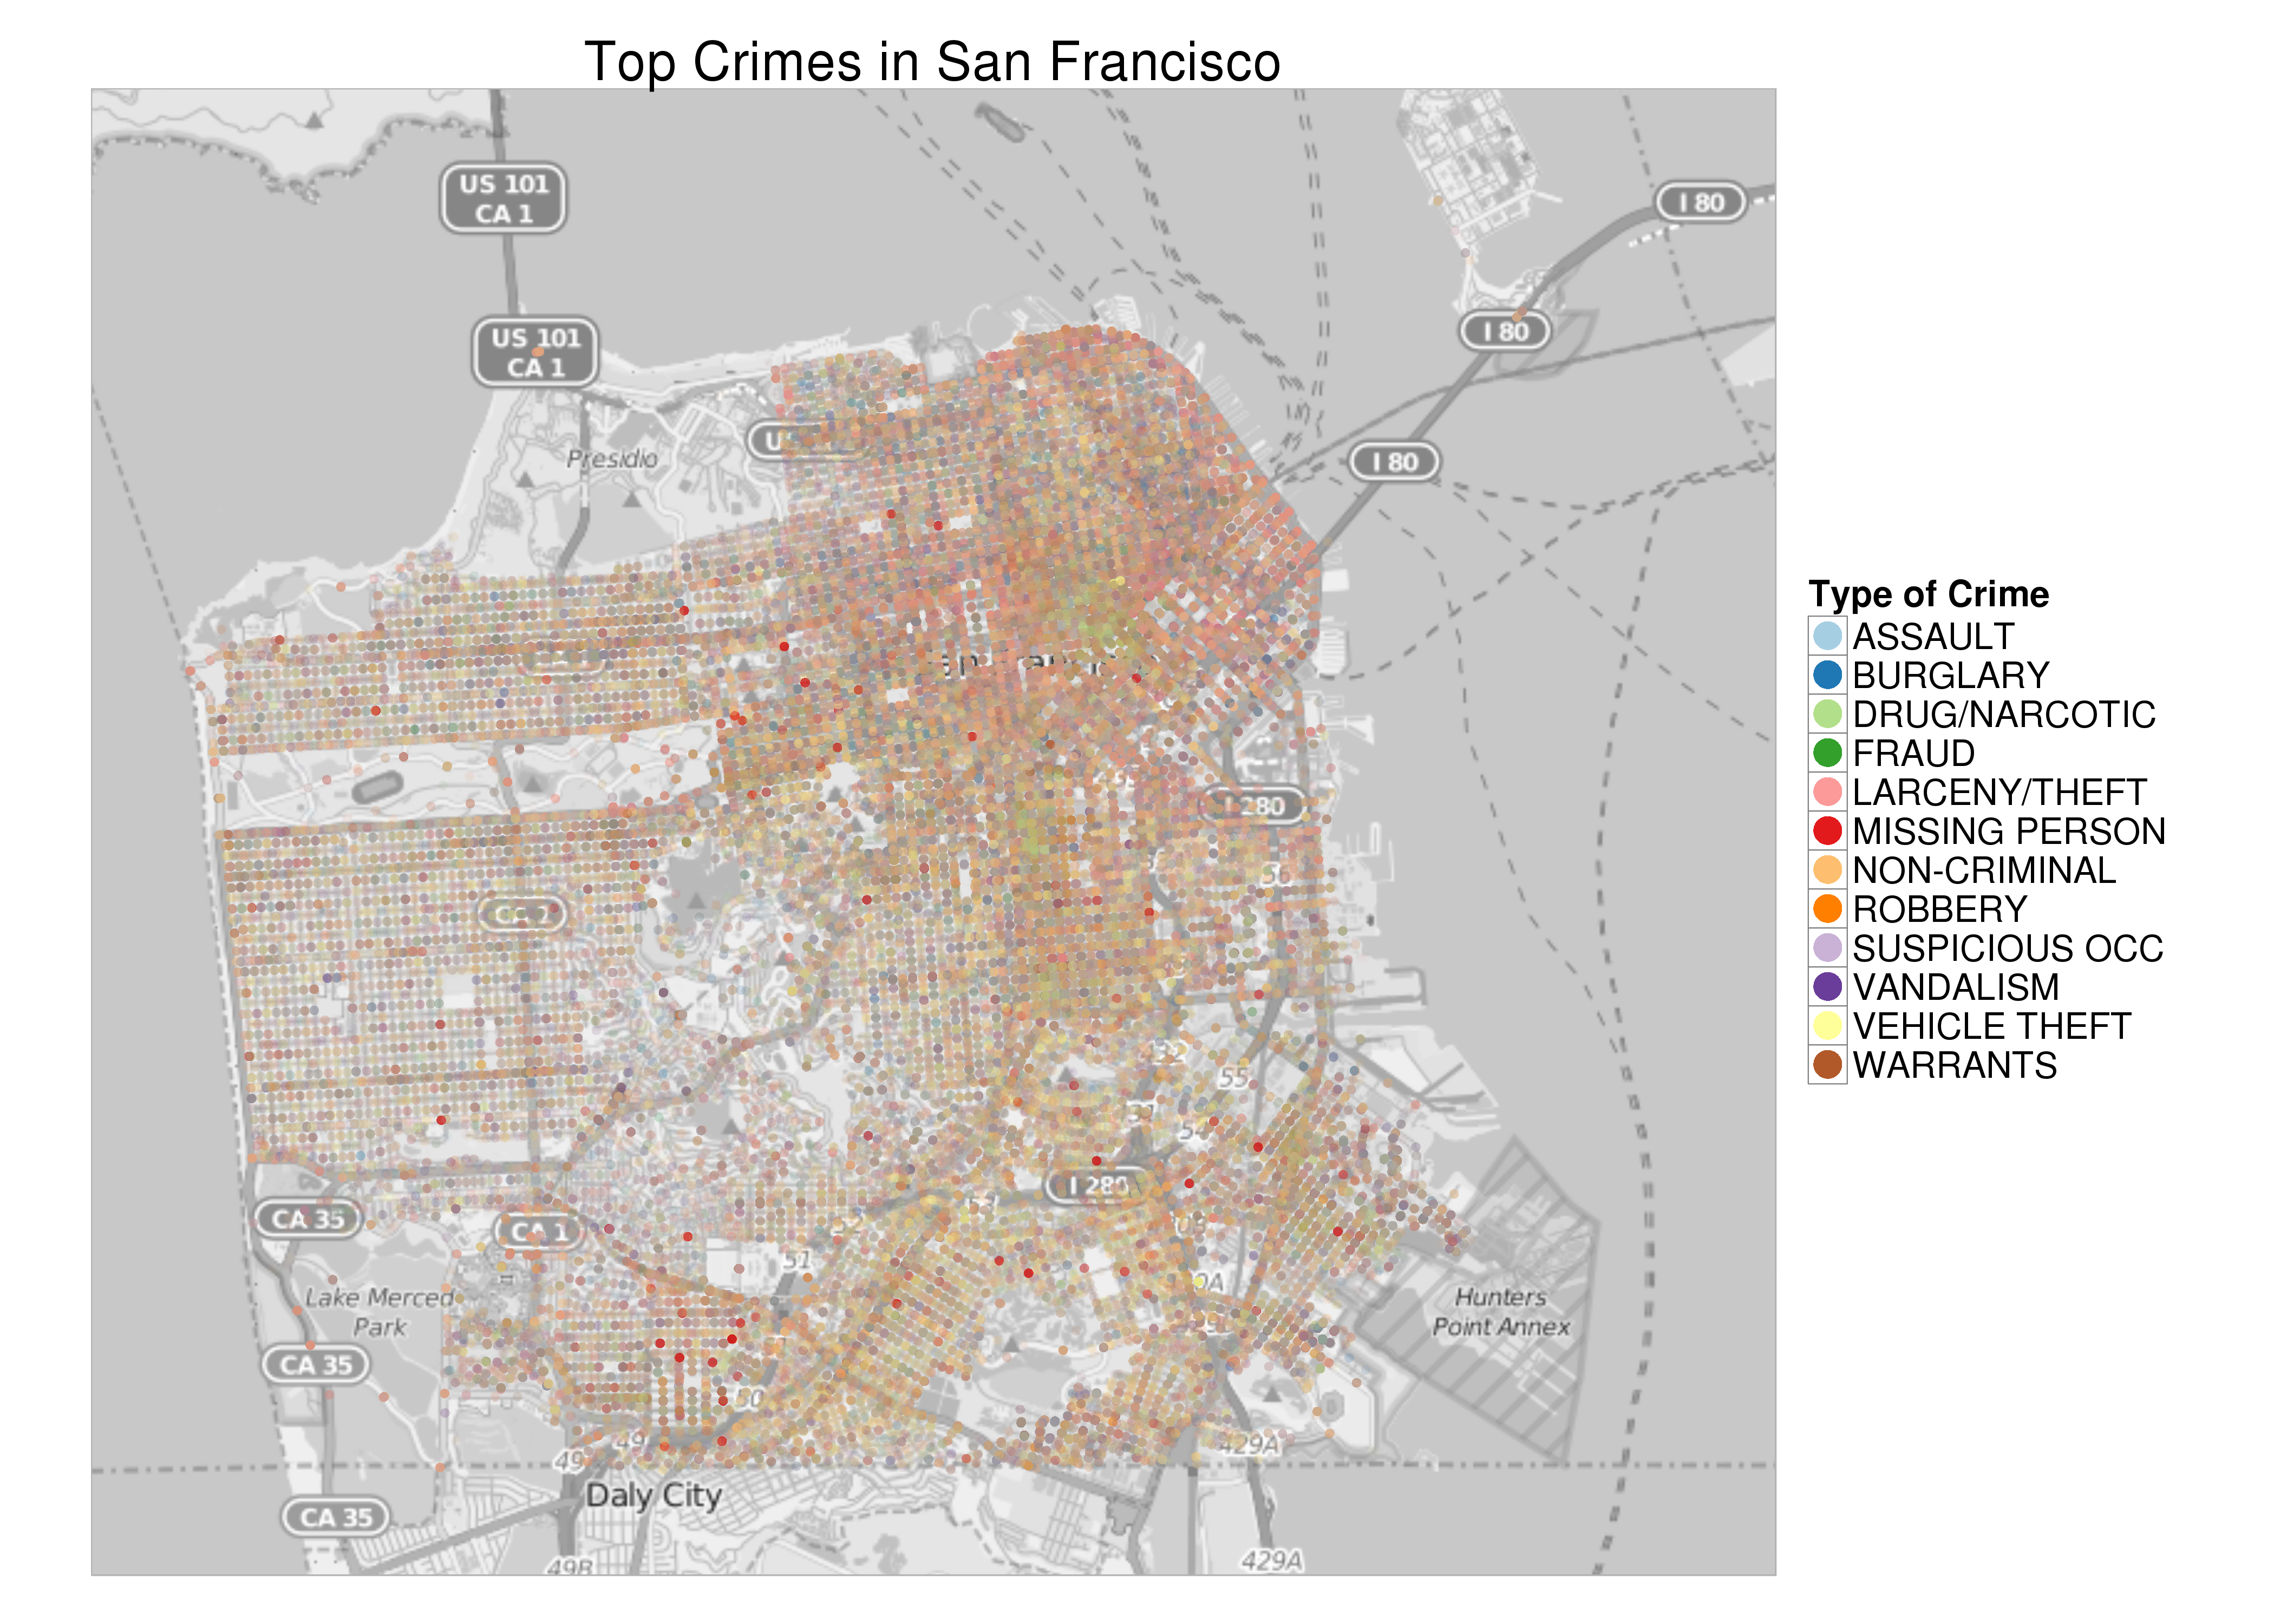
\includegraphics[width=\textwidth]{sf_top_crimes_map}
\caption{\cite{sf_crime_map}}
\end{figure}
\end{center}

\pagebreak
\section{Theoretical Principles}\label{s:theoretical_principles}
\subsection{Loss Function}\label{ss:loss_function}
The ranking of the results on the Kaggle leader board\citep{kgl_sf_crime} are based on the multi-class logarithmic loss function\footnote{The framework of \cite{keras} refers to the multi-class logarithmic loss function also as "categorical cross-entropy".}:

\begin{align}\label{eqn:loss}
&loss = -\frac1N\sum_{i=1}^N\sum_{j=1}^My_{ij}\log\left(p_{ij}\right)\\
\nonumber
N: & \hspace{8pt} \textrm{Number of cases in dataset.}\\
\nonumber
M: & \hspace{8pt} \textrm{Number of classes.}\\
\nonumber
y_{ij}: & \hspace{8pt} \textrm{Label for class. 1 if $i$ is in $j$. Otherwise 0.}\\
\nonumber
p_{ij}: & \hspace{8pt} \textrm{Predicted probability that $i$ belongs to $j$.}
\end{align}

This basically boils down to a format as follows:

\begin{center}
\begin{tabular}{c|c|c}
Class 1 & Class 2 & Class 3\\\hline
0.24 & 0.48 & 0.38
\end{tabular}
\end{center}

With the labels being:

\begin{center}
\begin{tabular}{c|c|c}
Class 1 & Class 2 & Class 3\\\hline
0.00 & 1.00 & 0.00
\end{tabular}
\end{center}

When those values are applied to \ref{eqn:loss}, we get a value of 0.49548. Of course, the closer the prediction is to the actual labels, the smaller the loss value will be.

To calculate examples quickly on the python console, the following code can be used:
\begin{lstlisting}[language=python,otherkeywords={as},label=lst:loglosscalculation,caption={Quick Log Loss Calculation in python}]
import numpy as np
from sklearn.metrics import log_loss
labels = np.array([0.0, 1.0, 0.0])
prediction = np.array([0.04, 0.78, 0.18])
print(log_loss(labels, prediction))
\end{lstlisting}


\pagebreak
\section{Methods}\label{s:methods}
\subsection{Dataset}\label{ss:dataset}
The Kaggle challenge \citep{kgl_sf_crime} provides 3 files on their site under "Data":
\begin{itemize}
\item \textbf{sampleSubmission.csv}(884k x 40): A sample file, demonstrating the expected format for submissions to the challenge. Consists of an array of the softmax prediction of each sample in the \textbf{test.csv}.
\item \textbf{test.csv}(884k x 7): The unlabeled sample subset of the data.
\item \textbf{train.csv}(878k x 9): The labeled sample subset of the data.
\end{itemize}
The data itself consists of the gathered crime reports of the San Francisco Police Department from January 1st 2003 through May 13th 2015, where the odd weeks belong to the \textbf{test.csv} and the even weeks to \textbf{train.csv}.

Here are the 10 first rows of the respective data files:

\begin{table}[htbp]
\centering
\setlength\tabcolsep{2pt}
\begin{tabular}{|cc|}\hline
Id&\textit{one column per class}\\\hline\hline
0&\textit{zeros, except the second last columns being all ones}\\
1&\vdots\\
2&\vdots\\
\vdots&\vdots\\\hline
\end{tabular}
\caption{sampleSubmission.csv(first 10 rows)}
\label{tab:sampleSubmission.csv}
\end{table}

\begin{table}[htbp]
\centering
\footnotesize
\setlength\tabcolsep{2pt}
\begin{tabular}{|ccccc}\hline
Id&Dates&DayOfWeek&PdDistrict&Address\\\hline\hline
0&2015-05-10 23:59:00&Sunday&BAYVIEW&2000 Block of THOMAS AV\\
1&2015-05-10 23:51:00&Sunday&BAYVIEW&3RD ST / REVERE AV\\
2&2015-05-10 23:50:00&Sunday&NORTHERN&2000 Block of GOUGH ST\\
3&2015-05-10 23:45:00&Sunday&INGLESIDE&4700 Block of MISSION ST\\
4&2015-05-10 23:45:00&Sunday&INGLESIDE&4700 Block of MISSION ST\\
5&2015-05-10 23:40:00&Sunday&TARAVAL&BROAD ST / CAPITOL AV\\
6&2015-05-10 23:30:00&Sunday&INGLESIDE&100 Block of CHENERY ST\\
7&2015-05-10 23:30:00&Sunday&INGLESIDE&200 Block of BANKS ST\\
8&2015-05-10 23:10:00&Sunday&MISSION&2900 Block of 16TH ST\\
9&2015-05-10 23:10:00&Sunday&CENTRAL&TAYLOR ST / GREEN ST\\\hline
\end{tabular}
\begin{tabular}{cc|}\hline
X&Y\\\hline\hline
-122.39958770418998&37.7350510103906\\
-122.391522893042&37.7324323864471\\
-122.426001954961&37.7922124386284\\
-122.437393972517&37.7214120621391\\
-122.437393972517&37.7214120621391\\
-122.45902362242902&37.7131719025215\\
-122.42561645123001&37.73935051446279\\
-122.41265203979201&37.739750156312105\\
-122.418700097043&37.7651649409646\\
-122.413934584561&37.798886450641604\\\hline
\end{tabular}
\caption{test.csv(first 10 rows)}
\label{tab:test.csv}
\end{table}

\begin{table}[htbp]
\centering
\scriptsize
\setlength\tabcolsep{2pt}
\begin{tabular}{|ccccc}\hline
Dates&Category&Descript&DayOfWeek&PdDistrict\\\hline\hline
2015-05-13 23:53:00&WARRANTS&WARRANT ARREST&Wednesday&NORTHERN\\
2015-05-13 23:53:00&OTHER OFFENSES&TRAFFIC VIOLATION ARREST&Wednesday&NORTHERN\\
2015-05-13 23:33:00&OTHER OFFENSES&TRAFFIC VIOLATION ARREST&Wednesday&NORTHERN\\
2015-05-13 23:30:00&LARCENY/THEFT&GRAND THEFT FROM LOCKED AUTO&Wednesday&NORTHERN\\
2015-05-13 23:30:00&LARCENY/THEFT&GRAND THEFT FROM LOCKED AUTO&Wednesday&PARK\\
2015-05-13 23:30:00&LARCENY/THEFT&GRAND THEFT FROM UNLOCKED AUTO&Wednesday&INGLESIDE\\
2015-05-13 23:30:00&VEHICLE THEFT&STOLEN AUTOMOBILE&Wednesday&INGLESIDE\\
2015-05-13 23:30:00&VEHICLE THEFT&STOLEN AUTOMOBILE&Wednesday&BAYVIEW\\
2015-05-13 23:00:00&LARCENY/THEFT&GRAND THEFT FROM LOCKED AUTO&Wednesday&RICHMOND\\
2015-05-13 23:00:00&LARCENY/THEFT&GRAND THEFT FROM LOCKED AUTO&Wednesday&CENTRAL\\\hline
\end{tabular}

\begin{tabular}{cccc|}\hline
Resolution&Address&X&Y\\\hline\hline
"ARREST, BOOKED"&OAK ST / LAGUNA ST&-122.425891675136&37.7745985956747\\
"ARREST, BOOKED"&OAK ST / LAGUNA ST&-122.425891675136&37.7745985956747\\
"ARREST, BOOKED"&VANNESS AV / GREENWICH ST&-122.42436302145&37.8004143219856\\
NONE&1500 Block of LOMBARD ST&-122.42699532676599&37.80087263276921\\
NONE&100 Block of BRODERICK ST&-122.438737622757&37.771541172057795\\
NONE&0 Block of TEDDY AV&-122.40325236121201&37.713430704116\\
NONE&AVALON AV / PERU AV&-122.423326976668&37.7251380403778\\
NONE&KIRKWOOD AV / DONAHUE ST&-122.371274317441&37.7275640719518\\
NONE&600 Block of 47TH AV&-122.508194031117&37.776601260681204\\
NONE&JEFFERSON ST / LEAVENWORTH ST&-122.419087676747&37.8078015516515\\\hline
\end{tabular}
\caption{train.csv(first 10 rows)}
\label{tab:train.csv}
\end{table}

The two datasets differ slightly in their columns. The training dataset has added the labels(Category) but also Descript and Resolution, which will be ignored for this project.

\begin{table}[htbp]
\centering
\scriptsize
\setlength\tabcolsep{2pt}
\begin{tabular}{|lll|}\hline
ARSON&ASSAULT&BAD CHECKS\\
BRIBERY&BURGLARY&DISORDERLY CONDUCT\\
DRIVING UNDER THE INFLUENCE&DRUG/NARCOTIC&DRUNKENNESS\\
EMBEZZLEMENT&EXTORTION&FAMILY OFFENSES\\
FORGERY/COUNTERFEITING&FRAUD&GAMBLING\\
KIDNAPPING&LARCENY/THEFT&LIQUOR LAWS\\
LOITERING&MISSING PERSON&NON-CRIMINAL\\
OTHER OFFENSES&PORNOGRAPHY/OBSCENE MAT&PROSTITUTION\\
RECOVERED VEHICLE&ROBBERY&RUNAWAY\\
SECONDARY CODES&SEX OFFENSES FORCIBLE&SEX OFFENSES NON FORCIBLE\\
STOLEN PROPERTY&SUICIDE&SUSPICIOUS OCC\\
TREA&TRESPASS&VANDALISM\\
VEHICLE THEFT&WARRANTS&WEAPON LAWS\\
\hline
\end{tabular}
\caption{Crime classes}
\label{tab:lables}
\end{table}
\pagebreak
The classes occur in an unbalanced matter: "Larceny/Theft" is the most predominant recorded crime, taking up nearly 19.92\% of the dataset. For this reason, 19.92\% is considered the bottom line of accuracy.
\pagebreak

\subsection{First Approach}\label{ss:first_approach}
For the first approach a \cite{keras} model on top of \cite{tensorflow} was chosen. For this, the first step was to pre-process the dataset to standardize it and properly feed it to the neural network.

\subsubsection{Pre-Processing}\label{sss:preprocessing1}
To handle CSV files properly, a \inlinelisting{CsvFile} class was created that represents a single csv file. When instantiated, it loads the csv file as a Pandas \inlinelisting{DataFrame}. Apart from an abstract \inlinelisting{def parse(self)}, it implements per-data-field functions that prepare the respective column for a conversion to a numerical representation(i.e. \inlinelisting{def _prepare_date(self, date: datetime)}). It also defines an export function \inlinelisting{def toNpArray(self) -> ndarray}, which allows to access the data as a \inlinelisting{numpy} array.

From this basic class, three other classes were derived:
\begin{itemize}
\item \inlinelisting{class TestDataCsvFile}\\
This class represents the \texttt{test.csv} file. It implements the missing \inlinelisting{parse(self)} method.
\item \inlinelisting{class TrainDataCsvFile}\\
This class represents the sample part of the \texttt{train.csv} file. It implements the \inlinelisting{parse(self)} method.
\item \inlinelisting{class TrainLabelsCsvFile}\\
This class represents the label part of the \texttt{train.csv} file. When instantiating, it can make a link to an already existing \inlinelisting{TrainDataCsvFile} class, to prevent loading the same csv file a second time. It implements the \inlinelisting{parse(self)} method.
\end{itemize}

All the \inlinelisting{CsvFile} derived classes support loading their already preprocessed data from the disk. This was implemented to reduce calculation time when performing multiple runs.

\paragraph{Feature Scaling and Mean Normalization}\label{p:feature_scaling_mean_normal}
Apart from converting the data into integers or floats, the \inlinelisting{_prepare_X} functions also perform feature scaling(usually to a $[-1, 1]$ set - sometimes $[0, 1]$) and mean normalization(i.e. the coordinates $X$ and $Y$).

\subsubsection{Keras Model}\label{sss:keras_model1}
To build the model, a dedicated \inlinelisting{Model} class was created. This class operates as a Keras model factory, using the \inlinelisting{get_model} to either create and train a model or load it's weights and parameters from a file and return the model.

The layers of the model changed greatly over time. This is the the last version of the model:

\lstinputlisting[language=python, firstline=28, firstnumber=28, lastline=41,label=lst:keras_model,caption={Keras model - model.py}]{../model.py}

\subsubsection{Classification process}\label{sss:classification_process1}
The classification process was written using the classes created in \ref{sss:preprocessing1} and \ref{lst:keras_model}(\ref{sss:keras_model1}):

\lstinputlisting[language=python, firstline=34, firstnumber=34, lastline=60,label=lst:main_py,caption={Classification process(first approach) - main.py}]{../main.py}

\subsubsection{Results}\label{sss:results1}
When using this setup, various settings did not raise the accuracy in any way. The accuracy value usually hovered barely below 20\%, which coincides with the bottom line described in \ref{ss:dataset} and could at best get to rank 1058. It was suspected that bad preprocessing of the dataset as well as the lack of knowledge and experience in neural networks was the cause for the lack of progress.

After various unfruitful tries, this approach had to be abandoned because of the lack in progress due to lack of knowledge and experience with Keras.

\pagebreak
\subsection{Second Approach}\label{ss:second_approach}
After an input from Prof. Yukawa, a new approach was established. This step consisted of using finished projects for this challenge as reference. For this, the project of \cite{efavdb_sf_crime_prediction} was chosen.

The system now relies on a Bernoulli Naïve Bayes classifier, which in contrast to the first approach \ref{ss:first_approach} does not require the system to build up layers to construct. It also uses a Logistic Regression algorithm to have a bar for comparison to be able to determine progress.

\subsubsection{Pre-processing}\label{sss:preprocessing2}
In this approach, the data was processed differently. To prevent the algorithm to search for patterns according to the principle of locality and simplify the data by binarization, columns were split up into several different dummy columns, namely:

\begin{itemize}
\item Minutes(m0 - m59)
\item Hours(H1 - H12)
\item Days(D1 - D31)
\item Months(M1 - M12)
\item Years(Y2003 - Y2015)
\item Weekdays(Monday - Sunday)
\item Districts(Bayview - Tenderloin)
\end{itemize}

\lstinputlisting[language=python, firstline=30, firstnumber=30, lastline=44,label=lst:newmain_py_preprocess,caption={Pre-processing method - newmain.py}]{../newmain.py}

\lstinputlisting[language=python, firstline=47, firstnumber=47, lastline=50,label=lst:newmain_py_evaluate,caption={Evaluation method - newmain.py}]{../newmain.py}

\lstinputlisting[language=python, firstline=53, firstnumber=53, lastline=82,label=lst:newmain_py_bnb,caption={Bernoulli Naïve Bayes fitting- newmain.py}]{../newmain.py}

\lstinputlisting[language=python, firstline=114, firstnumber=114, lastline=123,label=lst:newmain_py_lr,caption={Logistic Regression fitting - newmain.py}]{../newmain.py}

This lead to an expansion of the number of columns from 6 to 159, dropping column "Address" and binarizing all the other columns except for the coordinates, which remain floats.

\subsubsection{Results}\label{sss:results2}
This new classification system reached a value of 2.464 with the Bernoulli Naïve Bayes classifier. This log-loss value corresponds to an accuracy of 26.02\%. For comparison, the Logistic Regression reached 2.591 with an accuracy of 24.43\%. This result would correspond to rank 675 on the Kaggle leaderboard.

To finalize this project, it was decided to combine the findings of those two approaches to further advance in this challenge.

\pagebreak
\subsection{Third approach}\label{ss:third_approach}
Although the second approach \ref{ss:second_approach} was at an acceptable level, the failed first attempt was decided to be merged into the second one as comparison and to draw conclusions about what went wrong the first time. For this the classes written in the first approach were completely abandoned and only the core code of the first approach was amended and integrated into the script of \ref{ss:second_approach}.

\subsubsection{Results}\label{sss:results3}
The amended Keras model showed results on the same level as the Bernoulli Naïves Bays classifier from \ref{sss:classification_process1}. After a few tries, occasionally even slightly better results were reached:

\lstinputlisting[language=python, firstline=95, firstnumber=95, lastline=111,label=lst:newmain_py_keras,caption={Keras model integrated - newmain.py}]{../newmain.py}

With this configuration the model reached a log-loss of 2.456 (accuracy: 26.39\%), which was equivalent to rank 664. Which satisfies our definition of Done.

\pagebreak
\section{Results}\label{s:results}
Although the first approach lead to some measurable results(rank 1058), there were still many improvements to be made. Some of them were successfully implemented in the second approach and lead to an advance in rank to 675(log-loss: 2.464). After applying those findings into the first approach by merging both attempts, a further - although small - improvement could be made: The rank improved to 664(log-loss: 2.456).
\pagebreak

\section{Conclusion}\label{s:conclusion}
During this project, a number of mistakes have been committed. The biggest one was investing too much time into the first attempt, instead of looking up finished projects for reference. However, this is only clear now in hindsight, as at the point in time, no disadvantage could be identified. Nevertheless did this loss in time cause the project to halt at rank 664(log-loss: 2.456), instead of advancing further due to further research.

Another problem was the lack of knowledge on the part of constructing neural networks with APIs like Keras. This lead to a number of unnecessary attempts on improvement on the wrong front-line. Much time was spent on implementing the conversion from data into integer representation, feature scaling and mean normalization, even though later in the process(see \ref{sss:preprocessing2}) it turned out that binarizing the data was much faster in both programming and execution and brought better results.

\subsection{Future Considerations}\label{ss:future_considerations}
For future projects of similar nature, a better theoretical foundation is required. However, the mistakes made in this project were very insightful and helped in understanding general processes of creating neural networks.

If more time was available, the next step would have been enriching the dataset by relying on additional statistics and data from the internet. Other cited projects have relied on this method as well and just careless perusal makes this step seem very promising. The provided dataset by Kaggle after all only included date-time, district name and coordinates(address as well, but this was ignored in this project).

Another point to consider would be to process the data more: For example evening out distributions that otherwise are heavily uneven could lead to the neural network to not just abandon those samples in favour of sample types that are more prominent.

\pagebreak
\section{Listings}\label{s:listings}
\bibliography{reference}\label{bib}
\listoffigures\label{s:ListOfFigures}
\listoftables\label{s:ListOfTables}
\lstlistoflistings\label{s:ListOfListings}

\pagebreak
\appendix
\section{Appendix}\label{s:appendix}
\lstinputlisting[language=python,label=lst:main_py,caption={main.py}]{../main.py}
\lstinputlisting[language=python,label=lst:model_py,caption={model.py}]{../model.py}
\lstinputlisting[language=python,label=lst:preprocessor_py,caption={preprocessor.py}]{../preprocessor.py}
\lstinputlisting[language=python,label=lst:newmain_py,caption={newmain.py}]{../newmain.py}
\end{document}